\documentclass[letterpaper,11pt]{article}

\usepackage[margin=1.0in]{geometry}
\usepackage{amsmath}
\usepackage{amsthm}
\usepackage{amsfonts}
\usepackage{algorithm2e}
\usepackage{url}
\usepackage{fancyhdr}
\usepackage{blkarray}
\usepackage{graphicx}
\usepackage{csquotes}
\usepackage{cite}
\usepackage{caption}
\usepackage{subcaption}
\usepackage{placeins}

\pagestyle{fancy}
\lhead{Algorithmic-Trading Final Paper --- Fall 2018}
\rhead{}

\begin{document}
\thispagestyle{plain}
\noindent{Algorithmic-Trading Final Paper --- Fall 2018}

\noindent{Alex Thomas}

\noindent{Colgate University} \\

\noindent\textbf{Algorithmic-Trading Independent Study - Final Paper}

\section{Introduction}

The trading of stocks is one of the most important and prominent profit making utilities in the world. The introduction of 401k's into employment benefits has caused the majority of families in the United States to be invested in the stock market. Each portfolio has a unique distribution of owned stocks. Because of this, there is no way one person could possibly manage this - exposing the need for automation and computers. This is realized in mutual funds, which are collections of funds invested into a variety of different stocks, often compose large percentages of 401k portfolios. These funds often utilize algorithmic trading to produce maximum profit, motivating our study to understand how these strategies work. This has allowed millions of people to maximize longterm savings and retire far earlier \cite{Treleaven2013}.

To enter into the stock market one must purchase a particular number of shares of a particular security or mutual fund. This consists of companies, individuals, institutions, currencies, etc. However, this is a two-way transaction. To purchase a specific number of shares at a particular price, another party must agree to sell at least as many shares at that same price. This happens via broker or in modern times, via computer. From the trader's standpoint, it is as simple as logging onto a stock trading website and clicking execute trade. 

There are numerous different types of transactions in financial markets. Buying and selling of shares are some of the most common stock orders. {\it Limit orders} are buy and sell transactions that are only executed at a given limit price threshold. These orders are generally used to minimize loss and risk as trades will only occur when specific market conditions hold \cite{Aldridge2010}. {\it Shorting} of stocks works the opposite way of buying. With shorting, the trader is betting against the performance of the stock. The short sellers borrow shares of stock they don't own and sell them at market price. The goal is to re-buy the stock at a later date and return the borrowed shares to the lender by repurchasing the stocks at a lower price than the initial purchase. {\it Options trading} has gained recent popularity and is comprised of call and put options. This is a derivative type of security, as it is intrinsically linked to the price of something else. {\it Call options} give the owners the right to buy stock at a certain price, while {\it put options} gives the holder the right to sell stock at a certain price. Here, we are chiefly concerned with buying and selling transactions, however further study could examine some of the other types of orders mentioned above. 

 The intended outcome for any trade or transaction occurring is always the same: profit maximization. However, it is often difficult to pinpoint the exact moment in time that a particular trade maximizes profit. As computers and network connections have improved, trading financial instruments via automation has become more prominent. By using advanced mathematical models and measures, automated financial trading aims to maximize profit, executing up to thousands of trades a day of a particular security. While not often widely publicized, millions of trades each day are made by computer algorithms and not humans. In 2011, over 73\% of all equity trading volume in the U.S. was performed algorithmically \cite{Treleaven2013}. My study aims to analyze and study some of the most prominent algorithmic trading strategies.
 
 Rapid trading traces its roots back to the early 1930s. The stock market at its inception was entirely analog and trades of stock were carried out in person. Specialists and pit traders buying and selling positions at a physical location of the exchange and broadcasting it via telegram services \cite{Treleaven2013}.  Computerization of trades started in the 1980s when the NASDAQ introduced purely electronic trading. Today, trading time has changed from a matter of seconds to microseconds\cite{Treleaven2013}. The stock market moving entirely electronic gives motivation and reason for automated trading. Algorithmic Trading (AT) is therefore of critical importance, since it has been created in the early 1980s as the stock market was modernized. 

However, there have been some negative consequences from the adoption of algorithmic trading throughout the market. The May 6th, 2010 ``Flash Crash'' brought the public's attention to the little publicized, but very heavily used algorithmic trading in financial markets \cite{Kirilenko2017}. This happened with E-mini, denoted by ES, which is a stock market index futures contract that trades for around 50 times the value of the S\&P. A mutual fund complex sold 75,000 of these contracts valued at approximately $\$4.1$ billion - resulting in the largest net change in daily position of any trader in the E-mini since the beginning of the year. This caused a cascading effect, as other traders reacted to this massive momentary plunge and sold accordingly, with over 20,000 trades across 300 separate securities executing at prices 60 percent away from their initial prices a mere half hour earlier. The Dow Jones Industrial Average fell over 1000 points in a matter of moments, causing over \$1 trillion to evaporate within 10 minutes. 

AT is the generation and submission of orders of a financial asset by an algorithm, or set of instructions, that processes current market data and places orders in stock marketplaces without human interaction. More formally, Chaboud et al. define AT as: \begin{displayquote} ``In algorithmic trading (AT), computers directly interface with trading platforms, placing orders without immediate human intervention. The computers observe market data and possibly other information at very high frequency, and, based on a built-in algorithm, send back trading instructions, often within milliseconds. A variety of algorithms are used: for example, some look for arbitrage opportunities,
including small discrepancies in the exchange rates between three currencies; some
seek optimal execution of large orders at the minimum cost; and some seek to
implement longer-term trading strategies in search of profits.'' \end{displayquote} 

High Frequency Trading (HFT), is a subset of algorithmic trading and a far newer phenomenon that has been made possible by the rapid improvement of computerized trading speed \cite{Gomber2011}. This is the primary form of algorithmic trading found in financial markets today, with billions of dollars constantly traded by machines every second. 

\paragraph{} Here, we study the effectiveness of AT and HFT. AT is largely unregulated. There are absolutely no restrictions on electronic trading, which has resulted in instances of unstable performance throughout entire markets. Especially with the rise of costless transactions with platforms like Robinhood, it has never been easier for individuals to engage in AT. However, because the AT community is relatively secretive, our aim is to illuminate this area of financial trading. When properly executed, trading strategies can result in massive profits. 

\paragraph{} Furthermore, we give an in-depth analysis of a variety of both AT and HFT strategies. Specifically, we examine momentum, arbitrage and mean reversion measures and methods \cite{Aldridge2010}. While many of these methods can be applied to other financial markets, such as bitcoin markets, we use data exclusively from the US stock market. We develop a test suite that runs a variety of different algorithmic-trading strategies on two different periods of data. Some strategies which focus on HFT use intra-day, minute-by-minute stock data, while others look at a period of over 7 years of closing price data. By using different types of data, we are able to examine strategies in both an AT and a HFT context. 


\section{Preliminaries, Metrics, Measures}
In this study we examine numerous algorithmic trading methods. To measure the effectiveness of a particular strategy, we use a quality metric to analyze productivity. Different denominations of purchasing powers are used and compared against a {\it baseline measure}. The baseline measure is created by holding a long position of a specific denomination throughout the entire period of trading. Simply put, shares are bought at the beginning of the period and sold at the end. The profit level is then compared against the performance of the strategy. Much of the literature referenced actively studied the best performance of these strategies over different periods and used the same baseline comparison \cite{Liu2006}. Because this type of baseline position was used in a majority of the literature, it was necessary to include the same baseline in this study.

{\it Buy} and {\it sell signals} are thoroughly used throughout the study. Algorithms can generate a variety of buy and sell signals at a specific point in time, indicating that some denomination of stocks should be purchased or sold at that specific point in time. To measure how a given algorithm performs, different denominations of shares are purchased and compared. The strategies use closing price data from October 1st, 2006 to January 1st, 2017. Some strategies use intra-day stock data, which is minute-by-minute data of stock prices from October 26, 2018. Other additional terms need to be defined. {\it Securities} and {\it stocks } are used as terms interchangeably throughout the paper. Securities have more of a broad definition, as securities include stocks, bonds, mortgages, and others. {\it Bearish signals} signal trends of downturn whereas {\it bullish} signal positive, upwards trends \cite{Aldridge2010}. 

The stocks used in all strategies are found in Figure~\ref{stocktable}. These stocks were chosen to cover a variety of industries and markets to generate strong data. This is important because we need to account for different performances of stocks. Certain large tech stocks like FB or GOOG have had incredible trajectories and performances whereas other stocks outside of the tech industry like HAS, have performed more moderately. The range of stocks chosen encompass nearly all of the major industries throughout the world. Data was retrieved via Quandl, a financial data platform.

\begin{figure}[h]
\centering
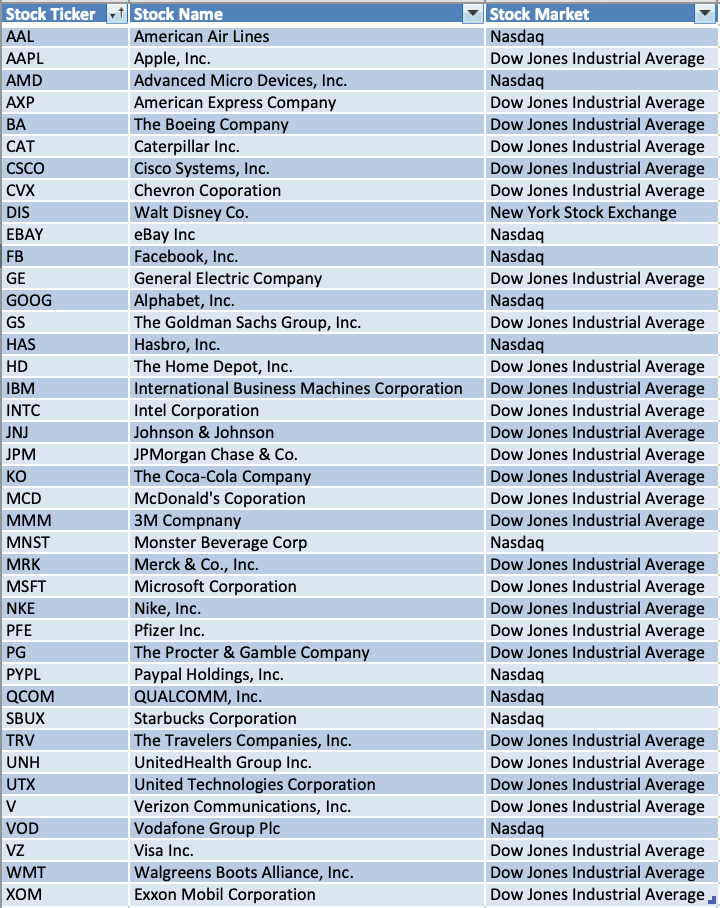
\includegraphics[width=85mm]{stock_table.png}
\caption{Table of stocks used in our study \label{overflow}}
\label{stocktable}
\end{figure}

For any given strategy, {\it windows} for strategies were chosen exclusively from the existing literature. A majority of the strategies used averages over a period of time, also known as {\it rolling averages}. For each strategy, the existing literature used different periods of time for the exact same rolling average. For the nature of the study, it makes sense to choose windows this way, as the goal was to identify and implement strategies to test effectiveness and not whether or not the industry standard windows were truly the best choice. Much of the literature referenced did extensive testing on the most effective strategy windows so it was prudent to incorporate these same windows in our experiments. However, it would be interesting in a future study to test how other windows performed. 

Graphs can be interpreted as follows. Figure~\ref{SMAfigure} shows the Simple Moving Average strategy applied to GOOG. Purple triangles, which are angled upwards, are buy signals while black triangles angled downwards are sell signals. On June 2015, the strategy generated a sell signal, denoted by the black triangle. In the following couple of months, a subsequent buy signal was generated as denoted by the purple triangle. The orange line is the long moving average, the blue line is the short moving average, and the red line gives the price of GOOG throughout the time. 

\begin{figure}[h]
\centering
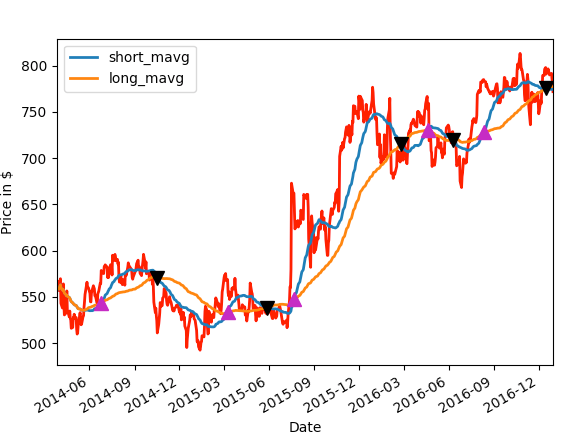
\includegraphics[width=90mm]{SMA_Google.png}
\caption{Simple Moving Average - "Golden Cross" Strategy applied to GOOG \label{overflow}}
\label{SMAfigure}
\end{figure}

\FloatBarrier

\section{Momentum Trading Strategies}

\subsection{Simple Moving Average}
Simple Moving Average (SMA) is an elementary AT measure. It is mostly used to measure average stock price over a period of time, however certain strategies solely rely on SMA. It looks at a rolling average of a specified window. Mathematically this can be defined as \cite{AlmeidaTeixeira}:  \[ SMA(t) = 1/n \sum_{i=t-n}^{t}x(i) \]  In words, this gets the average price over a specified window of time for a specified function. In the context of the stock market, SMA can be applied for both short term and long term averages, with the former under an hour while the latter can be hundreds of days or more. In application to the stock market and closing prices, this creates an average closing price for a specified amount of time, which gives an indicator of price swings in that period of time.

SMA is commonly leveraged into a strategy that uses a dual moving average \cite{AlmeidaTeixeira}. It works by taking two different SMA's - a short window and a long window. In our implementation, we chose a 40-day window and 200-day window, giving insight into a strategy that uses longer averages. The short window crossing below the long window gives a buy signal reinforced by high trading volumes. The long window crossing below the short window is considered bearish and gives a sell signal, as this signals that the stock is currently overvalued and will devalue. As demonstrated in Figure~\ref{SMAfigure}, the strategy generates 10 buy or sell signals over the period tested. Taking March 2015 as a specific example, buy signals are generated when the orange line - the long moving average, crosses the blue line - the short moving average, from below. Sell signals occur, like on June 2015, when the opposite occurs.

\subsection{Expected Moving Average}

Expected Moving Average (EMA) is closely linked to SMA. Like SMA, EMA functions over a rolling window; however, it is calculated differently. Mathematically, EMA is calculated with $F_i$ = the value associated with the moving average at period 0, $\alpha$ = smoothing constant, and $X_i$ = closing price of the security at period $i$ \cite{James1968}:  \[F_i = F_{i-1} +\alpha(X_i - F_{i-1})\]  In words, the EMA is found by multiplying the close subtracted by EMA from the previous day times a multiplier plus that prior day's average. This makes this measure far more weighted towards recent prices than SMA.

Like our implementation of SMA, EMA is commonly implemented with dual high and low value average. It takes two different EMA's, one with a low window and the second with a high window. However, because EMA reacts more closely to recent stock prices shorter windows are more commonly chosen. For our implementation, 12-day and 26-day windows were used. The short window crossing below the long window gives a buy signal reinforced by high trading volumes while the opposite is considered bearish and gives a sell signal. Figure~\ref{EMAfigure} demonstrates the EMA trading strategy applied to GOOG. Because smaller windows are used than our SMA implementation, we see far more buy and sell signals. Additionally, we see the short and long expected moving average lines follow the price line far closer than the SMA implementation.

\begin{figure}[h]
\centering
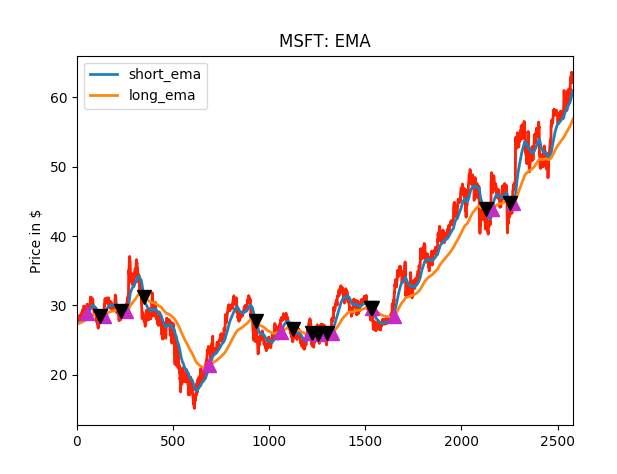
\includegraphics[width=90mm]{EMA_MSFT.png}
\caption{Dual Moving Average Strategy with Exponential effects applied to MSFT \label{overflow}}
\label{EMAfigure}
\end{figure}

\subsection{Bollinger Bands}

Bollinger Bands were introduced by John Bollinger in the 1980s\cite{Liu2006}. They provide a relative definition for high and low stock prices. This strategy uses 3 bands, with the 2 outer bands derived from a standard deviation of the moving average. Bollinger bands are great measures of market conditions of a particular security. Just like the previously examined techniques, the method uses a simple moving average as its basis, but instead incorporates 3 different bands separated by standard deviation. Because of this use of standard deviation, which is determined by market volatility, Bollinger Bands adjust themselves to market conditions. Precisely, the bands are calculated as follows with M - Middle Band, U - Upper Band, L - Lower Band, STD(x) - standard deviation of period x: \[M = SMA(12), U = M + 2 * STD(12),  L = M - 2 * STD(12)\] When the market is more volatile the bands widen and when the market becomes less erratic, the bands move closer together \cite{Liu2006}. Unlike the previous techniques, this strategy uses market conditions to evaluate trading orders.

This strategy is implemented with these 3 bands as mentioned above. For our implementation, a 12 day window was chosen to test out the algorithm, as this has been proven to be the most effective \cite{Liu2006}. When the closing price drops below the lower band, this gives a buy signal, as once a lower band has been broken due to heavy selling, the stock price will revert back and head towards the middle band. The opposite is true for when the closing price breaks the upper band, as this is indicative of heavy buying. The closing price approaching the upper band gives a bearish signal while approaching the lower band gives a bullish signal.  This strategy is showing in Figure~\ref{BBANDSfigure}. This measure can generate multiple buy or sell signals in a row. Looking at the first 100 days of the strategy, 5 straight sell signals are generated. The following 100 days subsequently generate 4 straight buy signals. This trend is indicative of the market giving only bearish indicators followed by a period of only bullish indicators stemming from the use of standard deviation in the measure.

\begin{figure}[h]
\centering
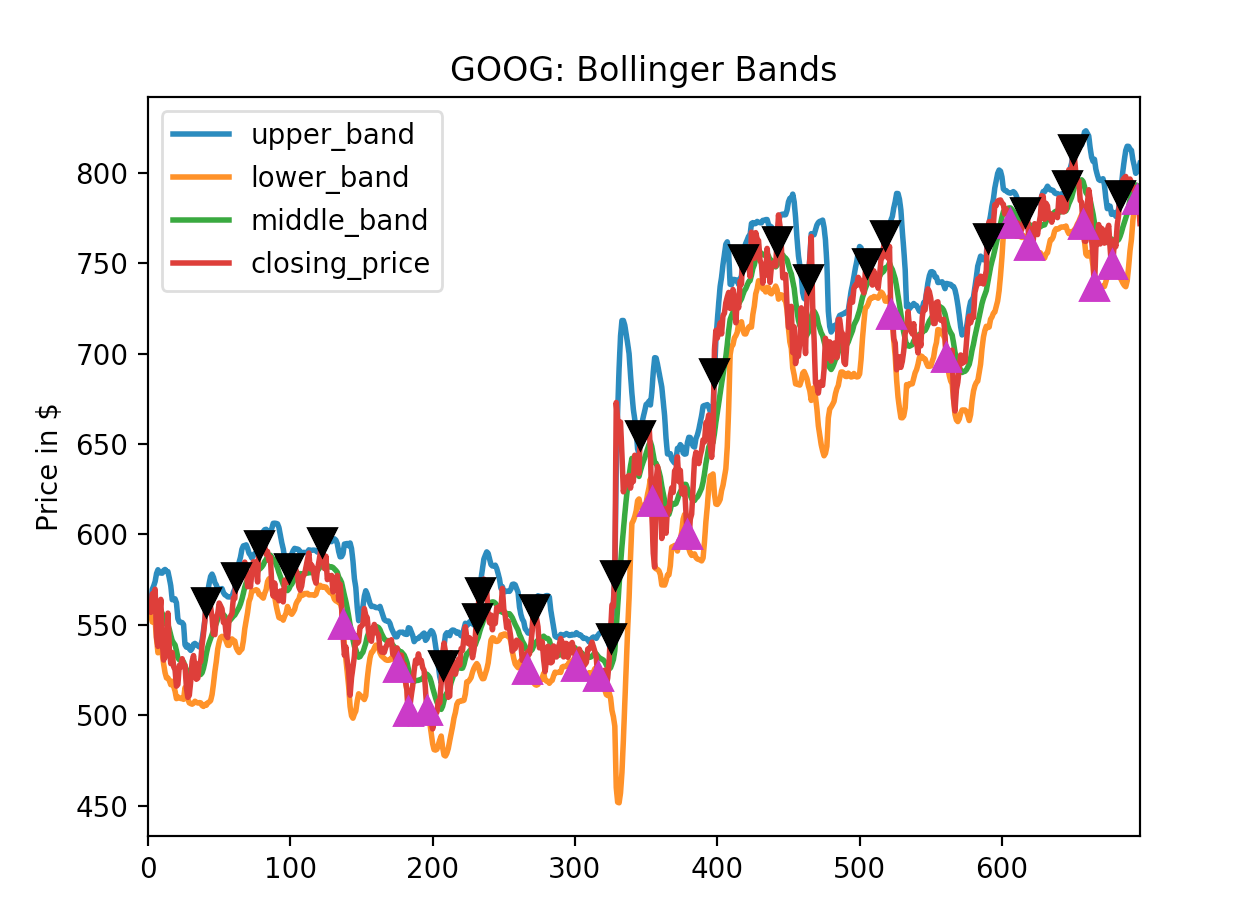
\includegraphics[width=90mm]{Goog_Bbands.png}
\caption{Bollinger Bands strategy applied to GOOG  \label{overflow}}
\label{BBANDSfigure}
\end{figure}

\subsection{RSI - Relative Strength Index}

Relative Strength Index (RSI) is a momentum indicator that measures the magnitudes of price changes to analyze overbought or oversold stocks. It demonstrates a particular security's recent performance over a relatively short window compared to the mean. This indicator is widely used today in algorithmic trading. The measure is a value between 0 and 100 at a specific date. The equation for RSI is as follows with $RS$ defined as average gain of up periods divided by the average gain of down periods over a specified window $x$ \cite{Chong2014}: \[RSI = 100.0 - (100.0 / (1.0 + RS(x))\] Therefore, a large RSI value is indicative of stocks that have had recent larger gains compared to losses while a low RSI value is indicative of stocks with poor recent performance compared to the mean.

This strategy takes advantage of mean reversion. Our implementation uses a very simple method. Sell signals are generated when the RSI is over 70 and buy signals are generated when the RSI is under 30 \cite{Chong2014}. This is very logical, as expected gains are the largest when a stock has performed poorly recently and is expected to revert back to the mean. This strategy also uses a 14 day window, which is standard across the industry. Figure~\ref{RSIfigure} shows this strategy when run on AAL. The second subfigure generates the buy and sell signals, as it shows the RSI of the stock throughout the period tested. These signals generated from the second subfigure are then plotted on the first subfigure over the stock price. Clearly, this strategy generates a large quantity of trading signals over the period.

\begin{figure}[h]
\centering

\begin{subfigure}[t]{0.45\textwidth}
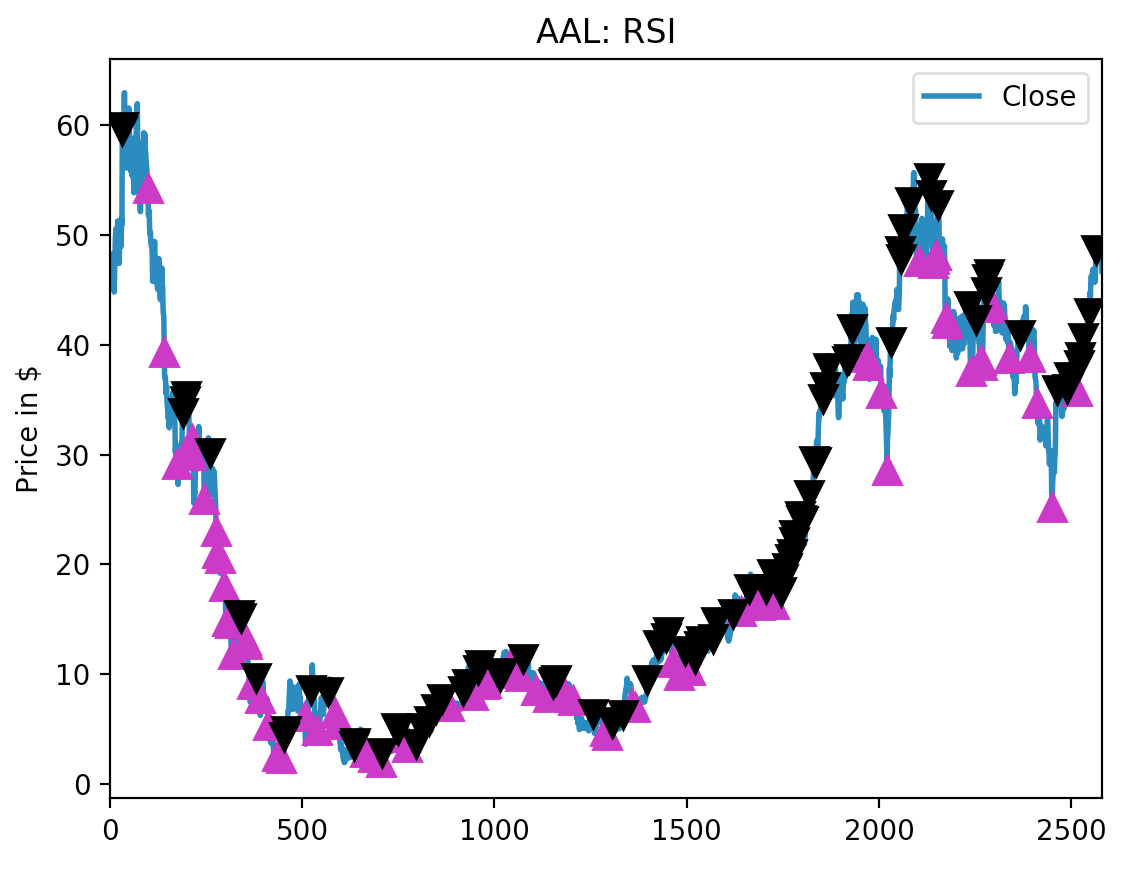
\includegraphics[width=\textwidth]{AAL_RSI_signals.png}
\caption{RSI Strategy \label{overflow}}
\end{subfigure}
\begin{subfigure}[t]{0.45\textwidth}
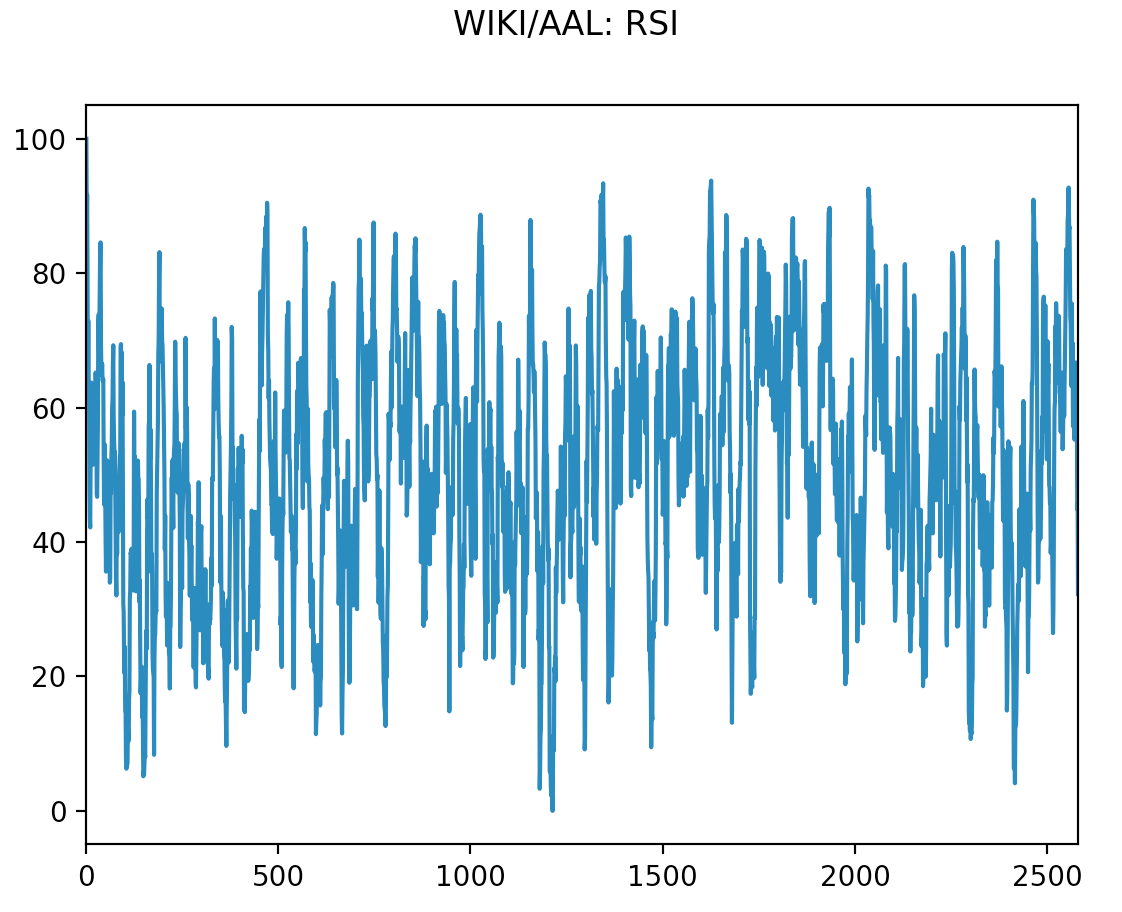
\includegraphics[width=\textwidth]{AAL_RSI.png}
\caption{ RSI of AAL \label{overflow}}
\end{subfigure}

\caption{RSI strategy applied to AAL  \label{overflow}}
\label{RSIfigure}
\end{figure}

\FloatBarrier

\subsection{Combining Momentum Indicators - RSI and Moving Average Convergence-Divergence (MACD)}

MACD uses two moving averages to identify trend changes while RSI performs exactly as stated in the above section. The MACD is constructed by subtracting two different sized exponential moving averages from each other. The equation for MACD is as follows and uses $EMA(x)$, with $x$ representing the period in minutes \cite{Chong2014}: \[ MACD = EMA(12) - EMA(16)\] The MACD is then plotted against a signal line, which is defined as S and is the EMA of the 9 minute MACD: \[ S = EMA(MACD(9)) \] Buy and sell signals are then generated by the ``golden cross" method. Specifically, this is when the MACD crosses the signal line from below - signaling a momentum swing and a bullish buy signal. A sell signal is the reverse - when the MACD crosses the signal live from above. Figure~\ref{RSIMACDfigure}a shows the MACD strategy applied to AAPL. This strategy behaves the exact same way as both Figure~\ref{EMAfigure} and Figure~\ref{SMAfigure}.

Unlike the previously mentioned strategies, this one combines indicators to generate more robust trading signals. Because there are two different measures working at the same time, buy signals are generated by both the RSI and MACD measures giving bullish signals within 3 minutes of each other. Sell signals are generated by either one of the measures producing a sell. Under this strategy, buy signals are very rarely generated while either strategy generating a sell denotes all shares to be sold. Because of the selectivity of buy signals, we can expect this technique to be very profitable. This strategy is most effective when run over intra-day data because of the relative infrequency of buy signals as demonstrated in Figure~\ref{RSIMACDfigure}b. Throughout an entire day, only 2 buy signals were generated. 

\begin{figure}[h]
\centering

\begin{subfigure}[t]{0.45\textwidth}
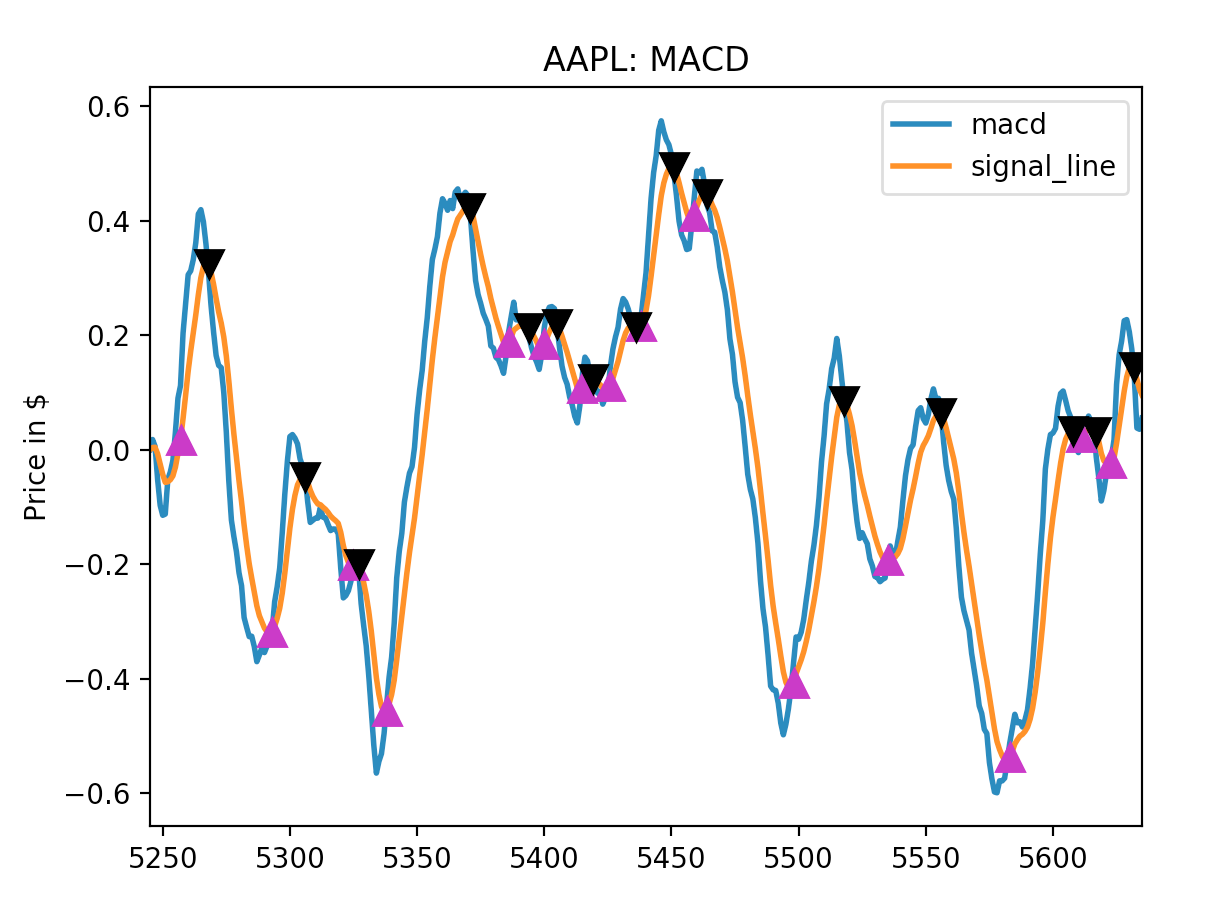
\includegraphics[width=\textwidth]{AAPL_MACD.png}
\caption{MACD Strategy \label{overflow}}
\end{subfigure}
\begin{subfigure}[t]{0.45\textwidth}
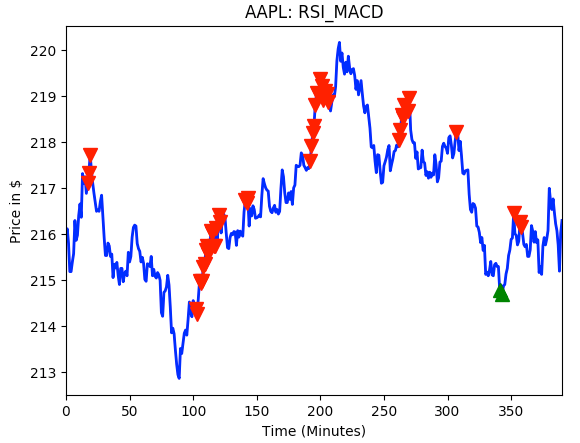
\includegraphics[width=\textwidth]{AAPL_RSIxMACD.png}
\caption{RSI and MACD strategy buy and sell signals \label{overflow}}
\end{subfigure}

\caption{RSI and MACD combination strategy applied to AAPL  \label{overflow}}
\label{RSIMACDfigure}
\end{figure}

\section{Pairs Trading - Arbitrage and Mean Reversion}

Pairs trading is an algorithmic trading strategy that chooses two economically linked stocks and profits off the divergence in spread of prices. Pairs trading uses statistical arbitrage, which is attempted profit from pricing inefficiencies identified through mathematical models. The most basic assumption is that prices will move towards their historical average, which pairs trading takes advantage of and is also known as mean reversion.  However, unlike other instances of mean-reversion, this strategy has a distinct advantage of always being hedged against market movements. 

Pairs trading is motivated by statistical arbitrage and mean reversion\cite{Fu2009}. When given two stocks that are linked economically (i.e. Pepsi and Coca-Cola), we expect the spread to remain relatively constant over time. However, there might be divergence in the spread between these two pairs cause by factors such as supply/demand changes or changes in volume in a particular stock.  Another problem with this is finding stocks that are closely related. Because we need to have stocks that behave similarly, we use cointegration to identify pairs of similarly behaving stocks. 

Cointegration is a stationary measure that highlights horizontal trends \cite{Gatev2006}. Unlike correlation, which only tracks similarly moving magnitudes over time, it instead tells how the difference between two regression lines changes over time. The implementation uses the python extension statsmodels to generate the p-value for cointegration. It is absolutely key to have related stocks, as this strategy takes advantage of mean reversion, or in other words, stocks reverting back to their original mean in relation to other similarly behaving ones. Now this is quite difficult, as it is very difficult to find stocks that are behave very similarly. After running comparisons of cointegration, certain tech stocks such as INTC and MFST were found to behave similarly.  

To generate trading signals, a Zscore is generated from the ratio of prices R(i) = ClosingPriceStockX/ClosingPriceStockY on a particular day $i$, the overall mean of ratio of prices M = AVG(R), and the standard deviation of the price ratio STD = STD(R): \[ Z = (R(i) - M)/STD\] The Zscore is a measure of how far away the current ratio of prices is away from its mean. Figure~\ref{PAIRSfigure}b shows the Zscore of both INTC and MSFT. Because of mean reversion, we can use this as a good indicator for buy and sell signals. A buy signal is generated when the zscore drops below -1, as we expect the zscore to return to its mean of 0. A sell signal is generated when the zscore goes above 1, as the stock is currently overvalued because we expect the stock to return to its mean of 0\cite{Fu2009}. These thresholds are shown in Figure~\ref{PAIRSfigure}b. In context of the pair of stocks, on buy signals the first stock in the pair is bought while the second is sold or shorted. The reverse is true on sell signals. Figure~\ref{PAIRSfigure} shows this strategy applied to INTC and MSFT. The red triangles represent sell signals while the green triangles show buy signals. Each time a buy signal is generated at a particular day the other stock has a matching sell signal and vice versa.

\begin{figure}[h]
\centering
\begin{subfigure}[t]{0.45\textwidth}
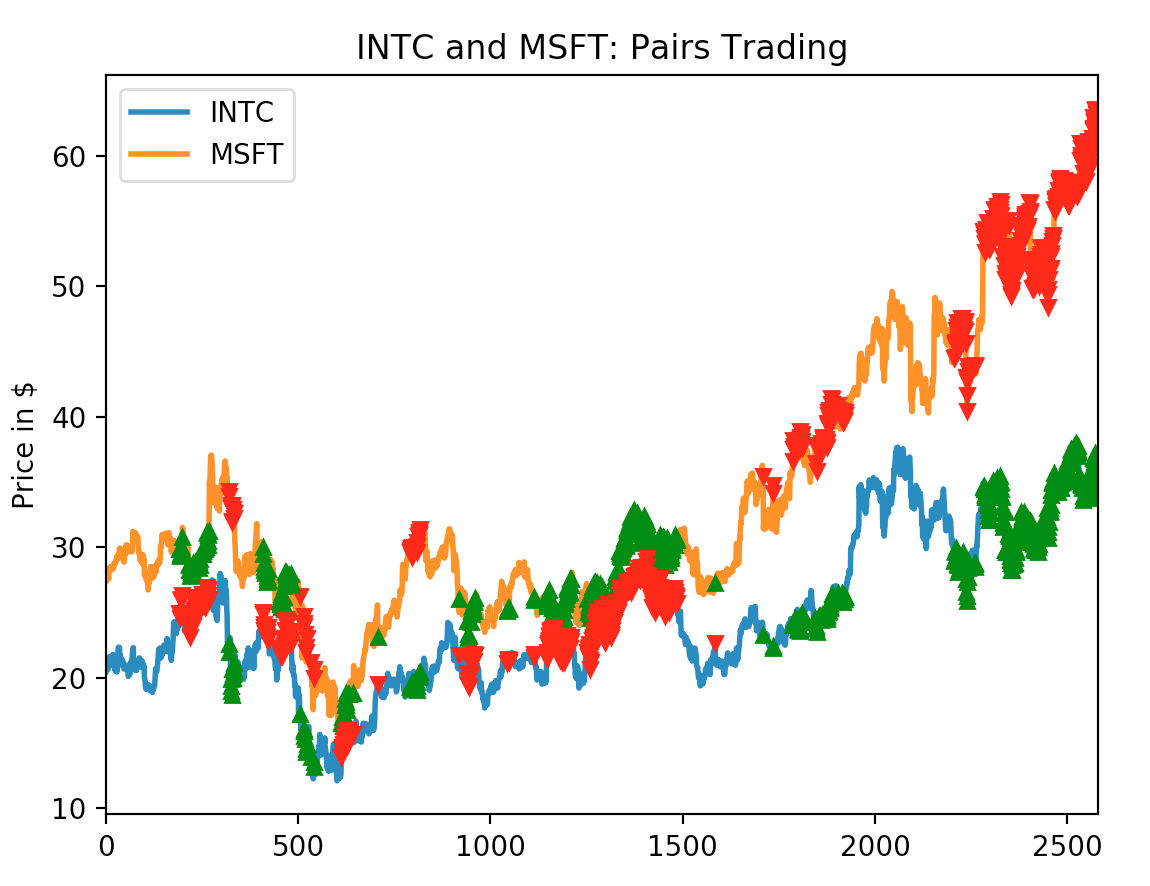
\includegraphics[width=\textwidth]{Intc_msft_signals.png}
\caption{Pairs Trading Strategy  \label{overflow}}
\end{subfigure}
\begin{subfigure}[t]{0.45\textwidth}
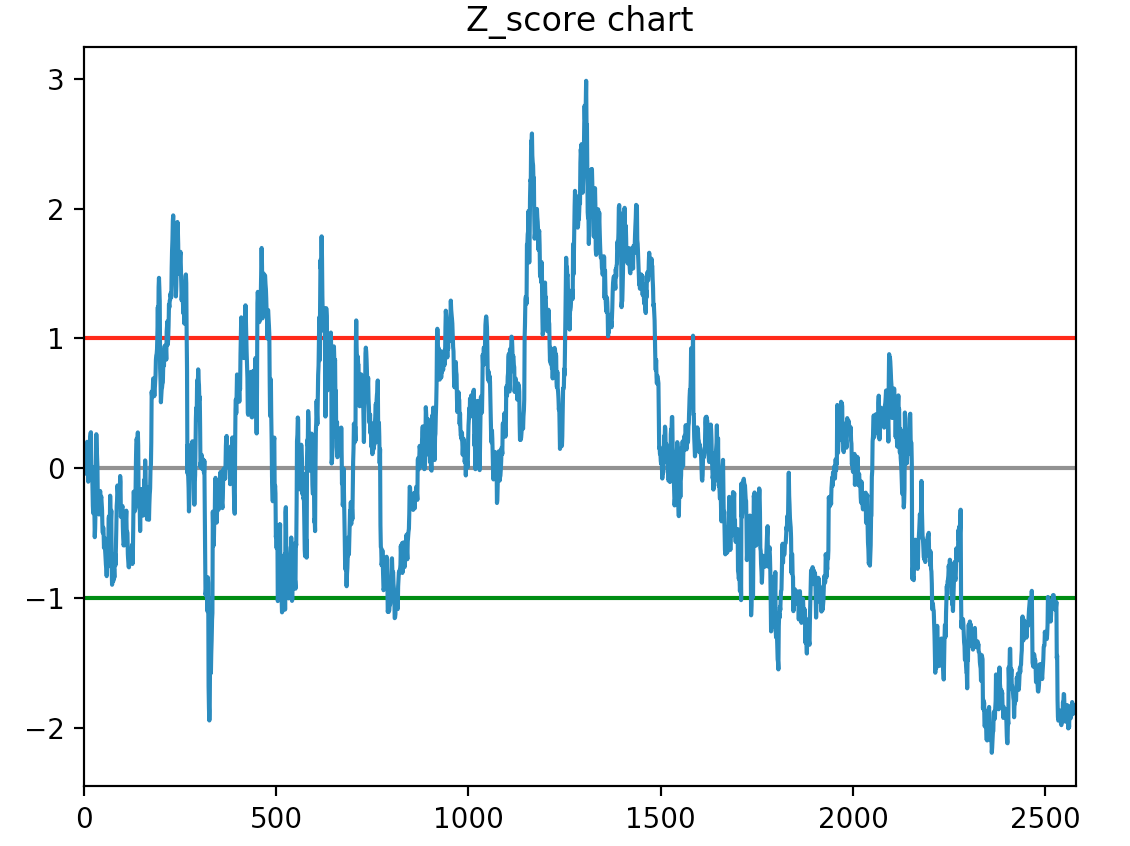
\includegraphics[width=\textwidth]{zscore.png}
\caption{Zscore of INTC and  MSFT \label{overflow}}
\end{subfigure}

\caption{Pairs Trading strategy applied to INTC and MSFT  \label{overflow}}
\label{PAIRSfigure}
\end{figure}

\FloatBarrier

\section{Results - Effectiveness and Analysis of Strategies}


The test suite runs all of the algorithms discussed above on a subset of stocks and generates profit figures for different denominations of stocks purchased. For every buy signal generated, the strategies ran on purchasing 10, 100, and 1000 stocks at a time. The strategies were implemented in Python and accessed stock data stored in csv files. The implementation leveraged Pandas Dataframes to store and manipulate the stock data. Pandas is a python data analysis package and is perhaps the most powerful open source data analysis or manipulation tool available. See Section 7.1 for pseudocode of each strategy's implementation.  The best way to understand how effective a particular strategy is to compare against a baseline, which is discussed above, helping us analyze the effectiveness of each strategy.   

\subsection{Momentum Strategies}

Standalone momentum strategies as a whole very rarely beat out the baseline measure. Figure 9 displays the results of AAPL, GOOG, HAS, QCOM, and AMD when using SMA, EMA, Bollinger Bands, and RSI. Only a few stocks had any strategies beat the baseline. One was GOOG, with both Bollinger Bands and RSI outperforming the baseline profit significantly. AMD for both SMA and EMA proved to be effective as well. However, for most it was more profitable to simply just buy and hold over the period. Figure~\ref{MOMENTUMfigure} demonstrates this poor performance. The baseline bar chart on the right side of the graph outperforms nearly every strategy. This however seems counterintuitive, as we should be generating profitable buying and selling trading signals with all of the computation, but that is clearly not the case.  Clearly, these strategies aren't viable as standalone trading algorithms. Now we will discuss why we observed overall poor performance.

The dual moving average algorithm when applied to both SMA and EMA isn't particularly effective. Due to the nature of SMA, which generally looks at long periods of time to highlight trends, this can induce a lagged effect to the buy and sell orders. A lagged effect in the context of moving averages is that the current moving average doesn't react to the current trend because of this longer observation window, often making this method ineffective. This lagged effect can be fixed by looking at an Exponential Moving Average analysis \cite{Ehlers}. However, unlike the literature suggests, in practice this doesn't translate to profit. AAPL nearly doubled its profit from using the exponential window that removes the lagged effect yet still had 2.53\% less returns than the baseline. While as a whole the strategy was more effective than SMA and did come closer to baseline performance, it rarely ended up beating it. This suggests that these indicators should be looked at in a different, combined context where multiple indicators could provide more robust trading signals. See the following section for discussion. 

With Bollinger Bands, buy and sell signals are still reliant on changes in rolling average prices. However, because of the incorporation of standard deviation, this strategy uses volatility in the market to further base buy and sell decisions. While a significant portion of the chosen stocks didn't end up actually out performing the baseline, a majority of them were within 1-2 percent performance of the baseline. 33\% of stocks tested on the strategy out performed each of its own baseline measure of buying and holding a specific denomination of shares throughout the entire period. Most notably, GOOG outperformed the baseline by 2.77\% while the implementations of SMA and EMA had abysmal performances of -30.25\% and -19.41\% respectively. While still not a passable standalone algorithm, the improvement over SMA and EMA is encouraging.

RSI takes advantage of over-purchasing or overselling of securities to predict convergence back to the mean. So, this strategy does take advantage of mean reversion. Unfortunately, most RSI implementations didn't outperform the baseline. The performance was comparable to EMA but slightly worse, as we see less stocks beating out the baseline. GOOG beat the baseline by 12.88\% while on the other hand DIS massively underperformed and posted a -7.08\% performance. 

\begin{figure}[h]
\centering
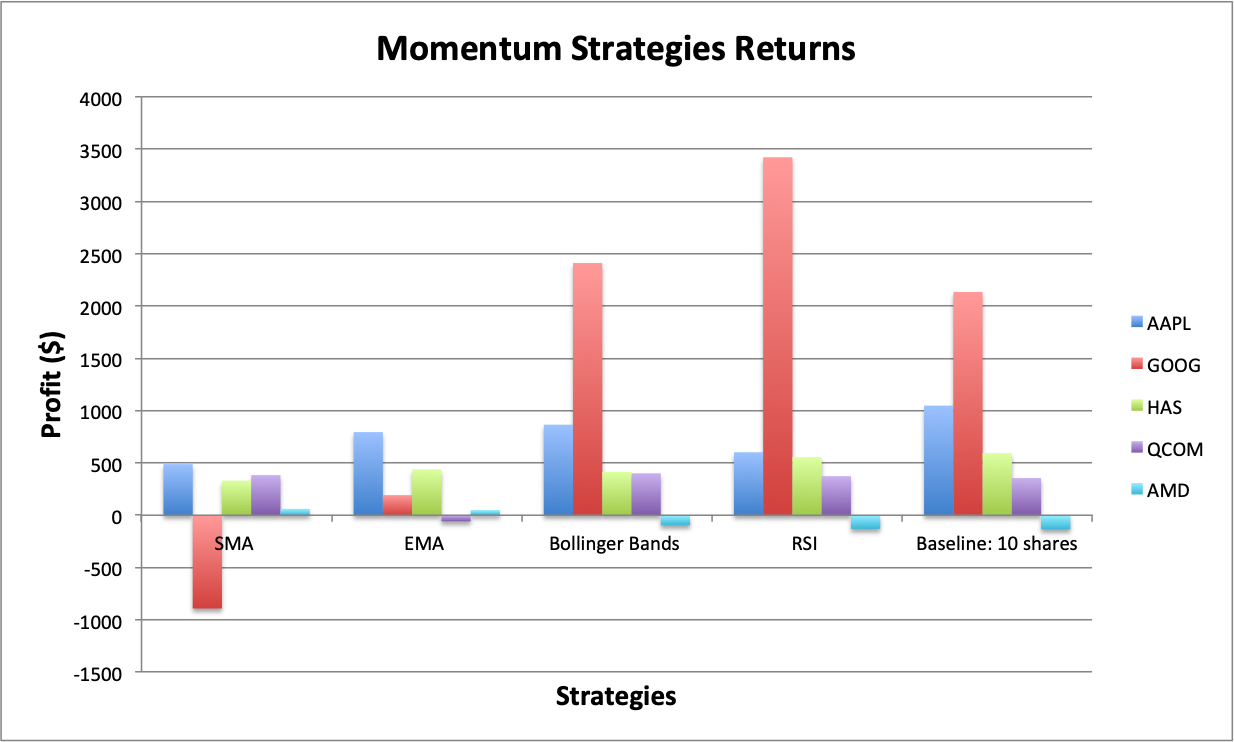
\includegraphics[width=.9\textwidth]{momentumstrategiesreturns.png}
\caption{Momentum Strategies Results  \label{overflow}}
\label{MOMENTUMfigure}
\end{figure}

\subsection{Combination Momentum Strategies}

The RSI and MACD combined implementation performed incredibly well. The most notable performances were from AAPL and HD. When purchasing 1000 shares at each buy signal, AAPL out-gained the baseline by \$9070  while HD had \$4990 of profit with the strategy while the baseline lost \$3750. Of all 30 stocks tested, only 3 stocks ended up with negative profit at the end of the day. AXP is a good example - generating a loss of \$1300 more than the baseline. With enough capital, this strategy could be used to generate incredible returns on a daily basis. Figure~\ref{RSIMACDRESULTSfigure} shows this strong performance. The green bar - the profit of the strategy buying or selling 1000 shares at a time, beats out the correspond baseline purple bar for every single stock, giving truly significant results. 

This algorithm generates incredibly robust buy signals and frequent sell signals which can nearly guarantee gains after buy signals. Therefore, utilizing strategies where 1000 shares of a given stock can generate massive profits with less risk of massive losses. It is also important that each transaction purchases a large amount of shares because it is necessary to offset the transaction cost charged by brokers. However, rather than focusing on individual stocks over time, this combination strategy is best implemented over a pool of multiple stocks because it isn't uncommon for days to generate absolutely no buy signals.

\begin{figure}[h]
\centering
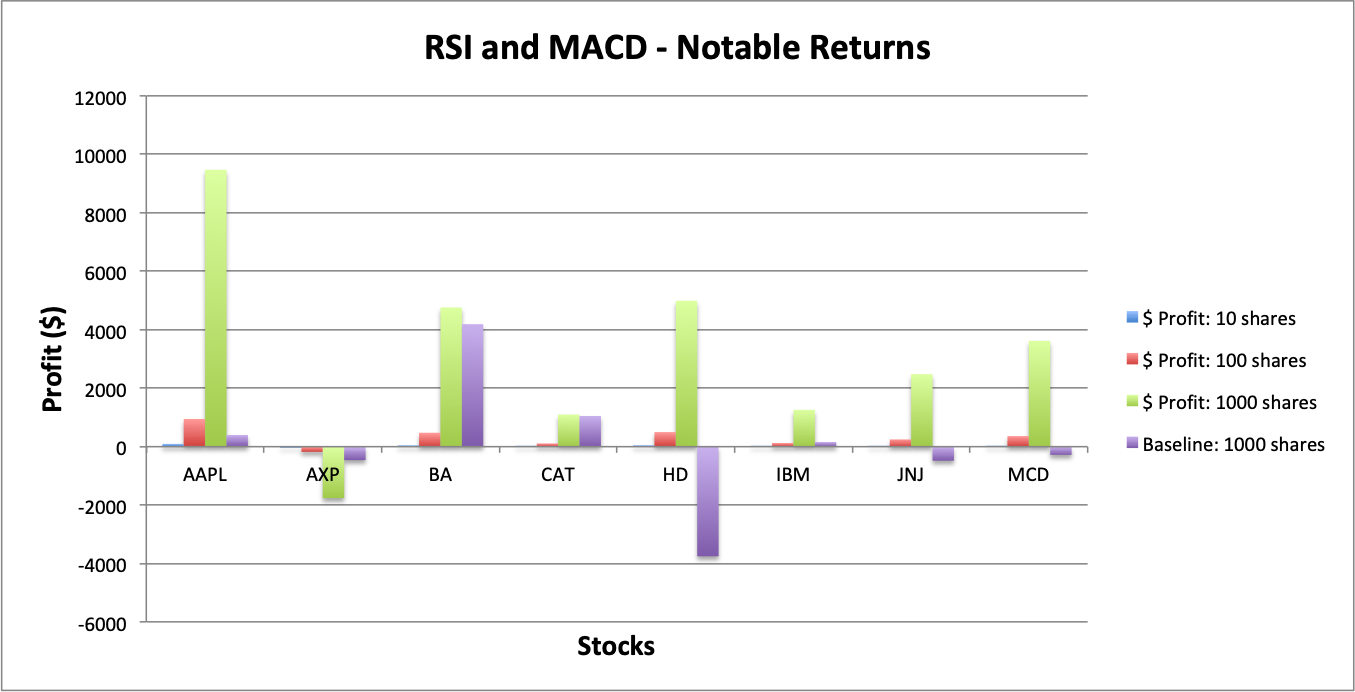
\includegraphics[width=.9\textwidth]{rsimacdresults.png}
\caption{RSI and MACD strategy   \label{overflow}}
\label{RSIMACDRESULTSfigure}
\end{figure} 

\subsection{Pairs Trading}

Just like the above strategy, our pairs trading implementation performed incredibly well. Compared against the baseline of SPY, a mutual fund that is the industry standard for baseline comparison of AT strategies, this strategy has amazing performance. When using AMD against SBUX, the strategy profited 2143.28\%. QCOM and SBUX performed similarly - culminating in 1748.06\% returns. However, even the lowest performing combination, AMD and VOD, beat out the baseline by over 138\%. Figure~\ref{PAIRSRESULTSfigure} shows these truly astounding results. Furthermore, this strategy would need to be tested on a larger pool of stocks, as only 5 combinations of stocks were cointegrated enough to justify trading together. 

This highlights a common trend. More involved strategies that use multiple measures or inputs always perform better than single measures and nearly always beat the baseline. Just like the combination momentum strategies, the results are incredible. With both pairs trading and as well as the above strategy, someone who implements either strategy could make incredible profits. The barrier to entry however for individuals to truly generate these massive profits, is being able to access up to the minute stock data. All data found via the internet or Quandl is delayed by upwards of 20 minutes, which can make the difference between thousands of dollars and profits and thousands of dollars of losses. However, because pairs trading uses closing prices, one wouldn't have to pay for the end of day closing data.

\begin{figure}[h]
\centering
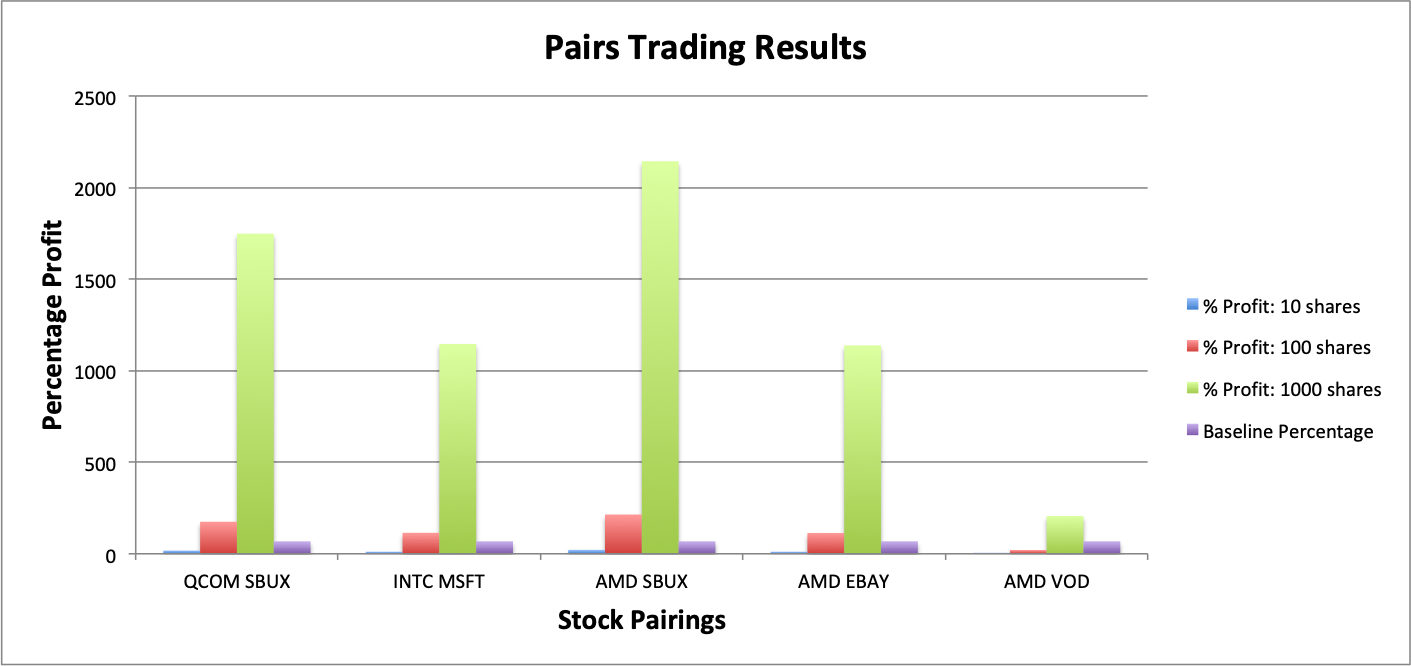
\includegraphics[width=.9\textwidth]{pairstradingresults.png}
\caption{Pairs Trading Results \label{overflow}}
\label{PAIRSRESULTSfigure}
\end{figure}

\section{Future Work}
Our work has been able to generate some high returns using existing algorithms and strategies. However, we have used exclusively mathematical models that have been entirely based on the stock price and volume. Other literature has examined using news- or media-content-based algorithmic trading as a profitable platform \cite{Zhang2010}. Surprisingly, this type of strategy has been found to be a viable indicator of stock market movement. However, there are no instances of researchers combining both mathematical- and news-sentiment-based trading strategies. Future work for a thesis would investigate a new trading algorithm combining both of the above strategies. The former would be implemented using the work done in this paper while the latter would be designed using Natural Language Processing (NLP) of Twitter data. Specifically, this would examine  publicly traded companies tweets using a combination of text sentiment and metrics such as favorites and retweets to generate buy and sell signals.


\section{Conclusion}

AT and HFT are far more secretive than I would have imagined. With the expansion of financial literacy and wide tools available today to trade over nearly every market now available to the average person, I would have expected a far more open-source, collaborative community that you find in the software/computer science field. 

SMA and EMA's application as a dual moving average strategy is a simple and naive AT strategy. However, many applications such as RSI and Bollinger Bands use moving average as its basis. Pairs trading and arbitrage strategies require much more involved implementation but are far more profitable. Other models that combine momentum indicators and applied as a HFT strategy are very successful as well. However, the barrier to entry for actually generating revenue for an individual is very high. Having lots of capital combined with up to the second stock data and transactional fees makes it very difficult for AT to be feasible for an individual. 

\section{Appendix}

\subsection{Implementation}

Included in this section is all of the pseudocode for the implementations described above.

\subsubsection{SMA}

\begin{verbatim}
def execute(stock, start_date, end_date):
    stock = stockDataRetriever(stock, start_date, end_date).getStock()

    # Initialize the short and long windows and buy sell in df
    short_window = 40
    long_window = 100
    
    # set Pandas df with stock data
    df = pd.DataFrame(index=stock.index)

    # Create short and long simple moving average 
    df['short_moving_average'] = df.movingWindow(short_window)
    df['long_moving_average'] = df.movingWindow(long_window)
    
    # mark signal based on comparison of the two averages
    df['signal'] = df.compare(short_moving_average, long_moving_average,1,0)
    
    # when signal changes from 1 to 0 or 0 to 1 - is a buy or sell
    df['positions'] = df['signal'].diff()

\end{verbatim}

\subsubsection{EMA }

\begin{verbatim}
def execute(stock, start_date, end_date):
    stock = stockDataRetriever(stock, start_date, end_date).getStock()

    # Initialize the short and long windows and buy sell in df
    short_window = 12
    long_window = 26

    # set Pandas df with stock data
    df = pd.DataFrame(index=stock.index)

    # Create short and long simple moving average
    df[short_exponential_moving_average] = df.ema(short_window)
    df[long_exponential_moving_average] = df.ema(long_window)

    # mark signal based on comparison of the two averages
    df[signal] = df.compare(short_exponential_moving_average, long_exponential_moving_average,1,0)

    # when signal changes from 1 to 0 or 0 to 1 - is a buy or sell
    df[positions] = df[signal].diff()

\end{verbatim}

\subsubsection{Bollinger Bands }

\begin{verbatim}
def execute(stock, start_date, end_date):
    stock = stockDataRetriever(stock, start_date, end_date).getStock()

    # Initialize the window
    window = 12

    # set Pandas df with stock data
    df = pd.DataFrame(index=stock.index)

    # Create the bollinger bands
    df['middle_band] = df.sma(window)
    df['moving_deviation'] = df.std(window)
    df['upper_band'] = df['middle_band'] + df['moving_deviation'] * 2
    df['lower_band'] = df['middle_band'] - df['moving_deviation'] * 2

    # mark signal based on when price moves above or below lower or upper bands
    df[signal] = df.compare((df_closing_price, df_lower band), 
    		     (df_closing_price, df_upper_band),1,0)

    # when signal changes from 1 to 0 or 0 to 1 - is a buy or sell
    df[positions] = df[signal].diff()

\end{verbatim}

\subsubsection{RSI }

\begin{verbatim}
def execute(stock1, stock2, start_date, end_date):
    stock = stockDataRetriever(stock1, start_date, end_date).getStock()

    # set Pandas df with both stocks
    df = pd.DataFrame(index=stock.index)

    # create measures of up and down performance
    delta = stock['Close'].diff()
    roll_up = delta[delta > 0].rolling.mean()
    roll_down = delta[delta > 0].rolling.mean()
    
    # create RSI
    RS = roll_up/roll_down
    RSI = 100.0 - (100.0 / (1.0 + RS))

    # create the buy and sell commands
    df['buy'] = np.where(RSI < 30, 1, 0)
    df['sell'] = np.where(RSI > 70, -1, 0)
    df['signal'] = df['buy'] + df['sell']

    # when signal changes from 1 to 0 or 0 to 1 - is a buy or sell
    df[positions] = df[signal].diff()

\end{verbatim}

\subsubsection{Combination Momentum Strategies }

\begin{verbatim}
def execute(stock, start_date, end_date):
    stock = stockDataRetrieverIntraday(stock, start_date, end_date).getStock()
	
    # create df for both RSI and MACD and merge
    rsi_df = RSI(name, stock)
    macd_df = MACD(name, stock)
    df = pd.merge(rsi_df, macd_df)
    
    # buy signals when both rsi and macd indicate buy
    # sell signals when either one of rsi or macd indicate sell
    df['buy'] = (df['signal_rsi'] == 1) & (df['signal_macd'] == 1)
    df['sell'] = (df['signal_rsi'] == -1) | (df['signal_macd'] == -1)
    df['signal] = df['buy'] + df['sell']

\end{verbatim}

\subsubsection{Pairs Trading}

\begin{verbatim}
def execute(stock1, stock2, start_date, end_date):
    stock_1 = stockDataRetriever(stock1, start_date, end_date).getStock()
    stock_2 = stockDataRetriever(stock2, start_date, end_date).getStock()

    # set Pandas df with both stocks
    df = pd.DataFrame(index=stock_1.index, stock_2.index)

    # create zscore from price ratios
    ratios = df['Close_stock1']/df['Close_stock2']
    zscore = (ratios - ratios.mean())/ np.std(ratios)

    # Create the buy and sell commands
    df['buy'] = np.where(zscore < -1, 1, 0)
    df['sell'] = np.where(zscore > 1, -1, 0)
    df['signal'] = df['buy'] + df['sell']

    # when signal changes from 1 to 0 or 0 to 1 - is a buy or sell
    df[positions] = df[signal].diff()

\end{verbatim}

\bibliographystyle{plain}
\nocite{*}
\bibliography{References}


\end{document}